%versi 2 (8-10-2016)
\chapter{Landasan Teori}
\label{chap:teori}
Pada bab ini akan dijelaskan mengenai konsep-konsep dasar pendukung PL, yaitu File Excel, iCalendar, JavaFX, Apache POI, iCal4j.

\section{Microsoft Excel}
\label{sec:excel}
Microsoft Excel atau Microsoft Office Excel adalah sebuah program aplikasi lembar kerja \textit{spreadsheet} yang dibuat dan didistribusikan oleh Microsoft Corporation yang dapat dijalankan pada Microsoft Windows dan Mac OS. Aplikasi ini memiliki fitur kalkulasi, pembuatan grafik.\cite{excel}

\subsection{Fitur Dasar}
\begin{figure}[H]
	\centering
	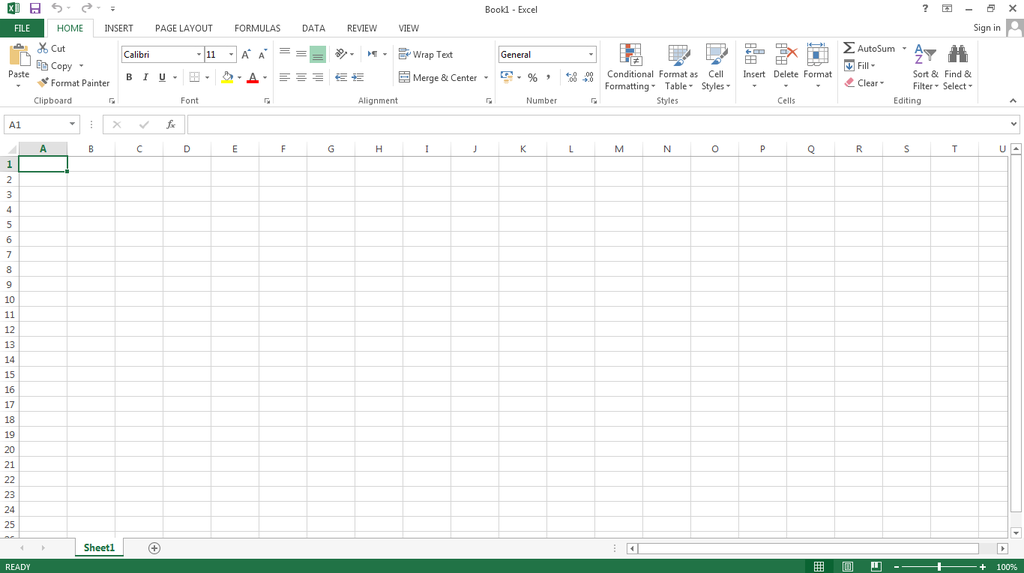
\includegraphics[scale=0.5]{Gambar/msExcel}
	\caption{\textit{Spreadsheet} Microsoft Excel}
\end{figure}
Microsoft Excel mempunyai semua fitur dasar dari \textit{spreadsheet}. MS(Microsoft) Excel memiliki sebuah grid dari sel yang diatur dalam beberapa kolom. Setiap kolom berisi huruf kapital yang berfungsi untuk mengatur atau memanipulasi data, contohnya operasi aritmatika. Terdapat beberapa fungsi atau rumus yang disediakan untuk membantu menjawab persoalan statistik, tehnik, dan kebutuhan keuangan. Sebagai tambahan, MS Excel dapat menampilkan data dalam \textit{line graph}, histogram dan chart.\cite{excel}

\subsection{Format File}
 Sebelum 2007 MS Excel memiliki paten dari format file biner yang dilamakan \textit{Excel Binary File Format}(.XLS). Pada tahun 2007 dengan penambahan XML maka format file dari excel berubah menjadi .xlsx . \cite{excel}

\section{iCalendar}
\label{sec:iCalendar}
iCalender merupkan format file komputer yang memungkinkan pengguna internet untuk mengirimkan undangan undangan pertemuan dengan pengguna internet lainnya dangan berbagai atau mengirimkan file dalam format yang memiliki ekstensi .ics .\cite{iCalendar}

\subsection{Komponen Utama}
Pada elemen bagian atas iCalendar terdiri dari rangkaian kalender, dan informasi penjadwalan. Sebuah informasi jadwal dapat berisi objek iCalendar tunggal maupun beberapa objek iCalendar yang buat group.\\
Baris pertama adalan BEGIN:VCALENDAR, dan baris terakhir berisi END:VCALENDAR, konten jadwal berada diantara kedua baris ini. Baris konten biasa disebut "\textit{icalbody}". Baris kedua merupakan versi format yang digunakan. Ada dua versi dari vCalendar yaitu VERSION:1.0 dan VERSION:2.0. Bodi dari objek iCalendar terdiri dari list properi kalender dan satu atau lebih komponen kalender. Properti dari kalender dapat di aplikasikan ke seluruh kalender. Komponen Kalender terdiri dari beberapa properti kalender untuk membuat sebuah skema kalender(desain). Misalnya, komponen kalender dapat menentukan sebuah event, daftar to-do, sebuah entri jurnal, informaasi zona waktu, informasi waktu sibuk/lenggang, atau sebuah alarm. \\
Berikut ini contoh dari sebuah objek iCalendar. Obek iCalendar ini berisi hari ulang tahun bastille yang dilaksanakan pada 14 juli 1997, pukul 17:00(UTC) sampai 15 juli 1997, pukul 03:59(UTC).\cite{iCalendar}
\begin{figure}[H]
	\centering
	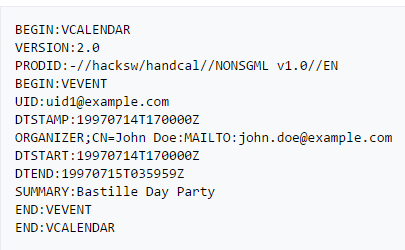
\includegraphics[scale=0.5]{Gambar/CaptureiCalendar1}
	\caption{Contoh iCalendar}
\end{figure}

\subsection{Event(VEVENT)}
VENVENT menggambarkan sebuah event yang dijadwalkan dengan rentang waktu tertentu. Sebuah VEVENT memili DTSTART untuk menetapkan waktu awal, dan DTEND menetapkan waktu akhir dari sebuah event.\cite{iCalendar}
\begin{figure}[H]
	\centering
	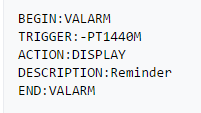
\includegraphics[scale=0.5]{Gambar/CaptureiCalendarEvent}
	\caption{Contoh VEVENT pada iCalendar}
\end{figure}

\subsection{Tipe Komponen Lain}
Terdapat komponen lain pada iCalendar, yaitu VTIMEZONE (zona waktu) and VALARM (alarm). VTIMEZONE  menerangkang zona waktu pada kalender. VALARM untuk memasang alarm pengingat pada kalender. UID merupakan tanda pengenal yang membuat kalendar. \cite{iCalendar}



\section{Apache POI}
\label{sec:apache} 

Apache POI(\textit{Poor Obfuscation Implementation}) pada hakikatnya merupakan \textit{library} untuk memanipulasi dan menciptakan sesuatu melalui Java API( \textit{application programming interface}) dengan memanipulasi berbagai format file berdasarkan \textit{Office Open XML standards}(OOXML) dan dokumen \textit{Microsoft OLE 2 Document Compound Format}(OLE2), Singkatnya dengan library ini memungkinkan untuk membaca dan menulis pada MS Excel menggunakan Java.\cite{apachepoi} \\


\subsection{Komponen Apache POI}
\label{subs:komponen} 
Untuk membaca aplikasi MS Office Apache POI mempunyai modul berisi komponen java api untuk membaca dokumen dengan format OLE2 dan OOXML. Berikut ini komponen-komponen dalam Apache POI.\cite{apachepoi}  

\begin{enumerate}
	\item Excel \textit{workbooks} (HSSF dan XSSF)
	\item Word \textit{document} (HWPF dan XWPF)
	\item PowerPoint \textit{presentation} (HSLF dan XSLF)
	\item Outlook (HSMF)
	\item Visio (HDGF dan XDGF)
	\item Publisher (HPBF)
\end{enumerate}

HSSF merupakan singkatan dari \textit{Horrible Spreadsheet Format}, sedangkan XSSF merupakan singkatan dari \textit{XML Spreadsheet Format}. HSSF dan XSSF memberikan cara untuk membuat, membaca, dan memodifikasi XLS spreadsheet. Pada sub bab ini akan difokuskan untuk membahas XSSF sesuai kebutuhan untuk menganalisa file excel jadwal mengawas ujian yang dikeluarkan oleh TU FTIS.\cite{apachepoi}


\subsection{Kelas Inti Apache POI}
\label{subs:kelas_inti}

\begin{figure}[H]
	\centering
	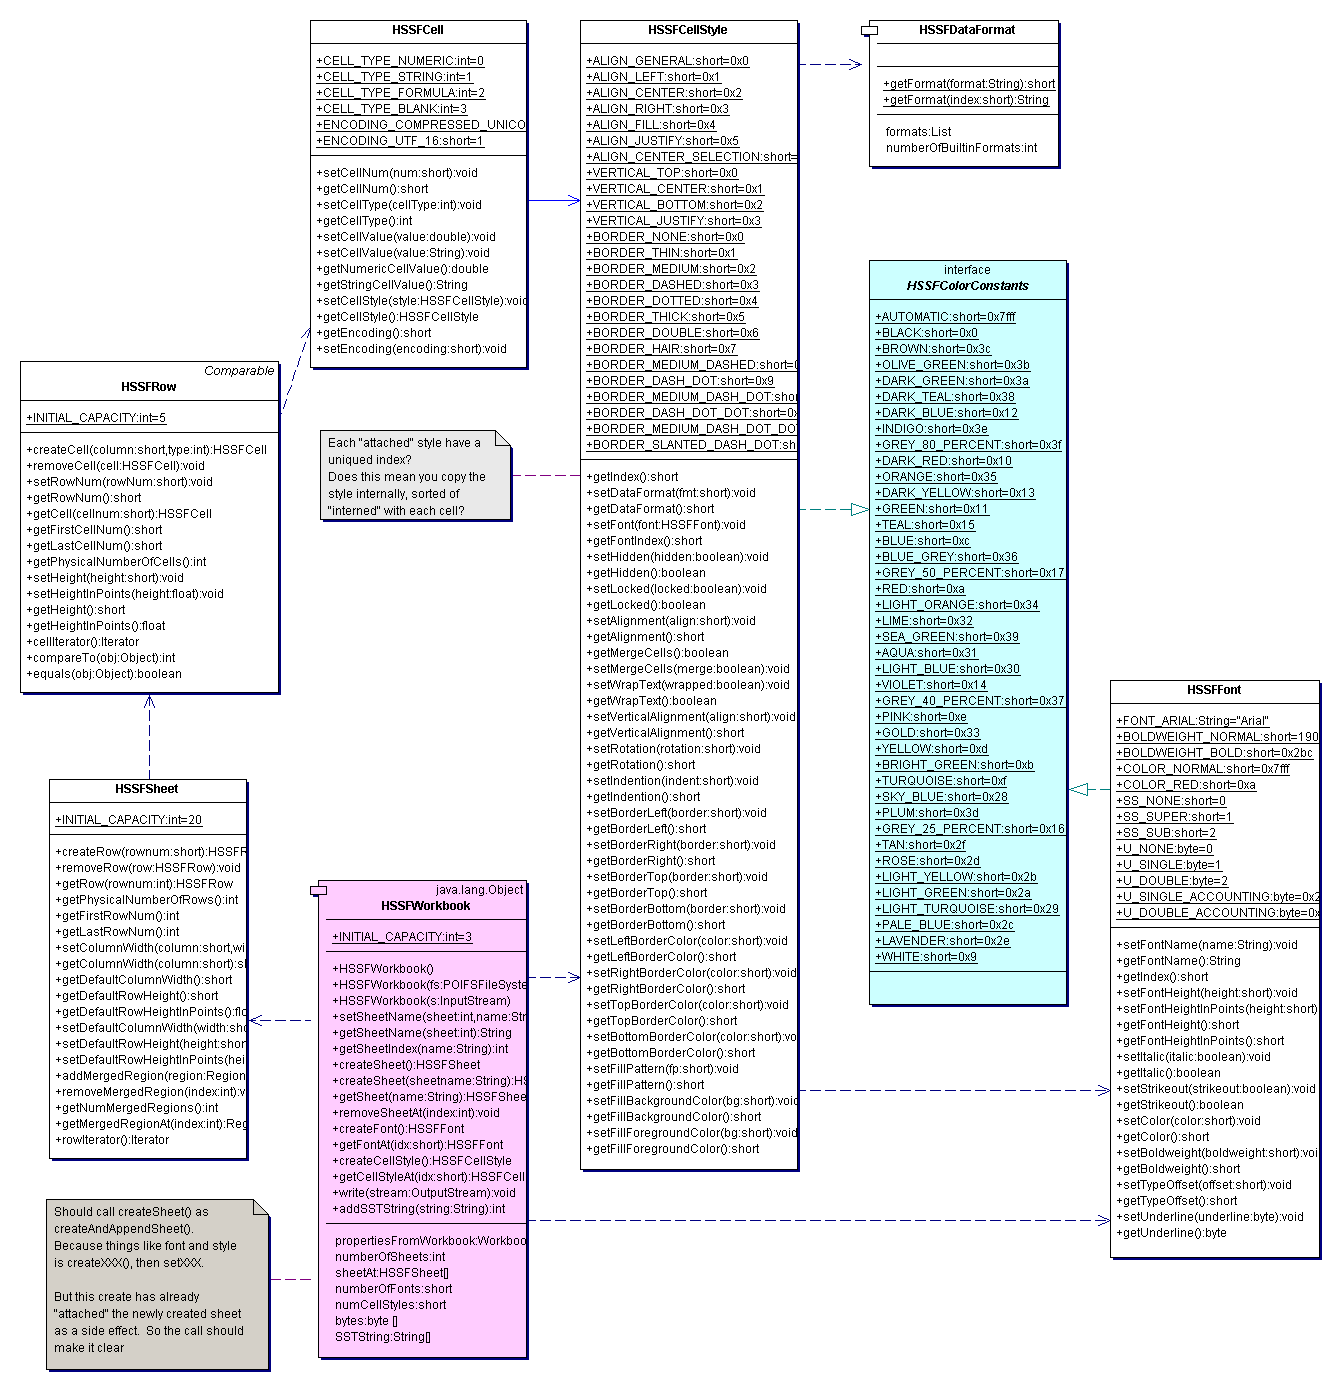
\includegraphics[scale=0.3]{Gambar/hssf}
	\caption{Kelas diagram hssf}
\end{figure}

Pada sub bab ini akan membahas introduksi mengenai beberapa kelas dan method yang ada di Apache POI API yang merupakan bagian penting untuk bekerja dengan file excel mengunakan program Java. Kelas HSSF dan XSSF mempunyai struktur kelas yang sama yang membedakan adalah kompatibilitas versi format excel yang dapat dibaca. \cite{apachepoi2}

\subsubsection{Workbook}
\label{subs:workbook} 
\textbf{org.apache.poi.ss.usermodel} \textit{package} merupakan \textit{super-interface} dari semua kelas yang berhubungan dengan pembuatan atau me-\textit{maintain} Excel workbook. Dua kelas yang mengimplementasikan \textit{interface} tersebut sebagai berikut:\cite{apachepoi2}

\begin{itemize}
	\item \textbf{HSSFWorkbook} : Kelas ini mempunyai method yang dapat membaca dan menulis file Microsoft Excel dengan format .xls. Kelas ini kompatibel dengan MS-Office versi 97-2003.
	\item \textbf{XSSFWorkbook} : Kelas ini mempunyai method untuk menulis dan membaca Microsoft Excel dan OpenOffice xml dengan format .xlsx. Kelas ini kompatibel dengan MS-Office versi 2007 atau versi barunya.
\end{itemize}  

\subsubsection{XSSFWorkbook}
\label{subs:XSSFWorkbook}
Kelas ini merepresentasikan baik \textit{high} dan \textit{low} level format file excel. XSSFWorkbook merupakan kelas yang berada dalam \textit{package} \textbf{org.apache.xssf.usermodel} dan mengimplementasikan antarmuka workbook. Berikut ini list method dan constructor dalam kelas ini.\cite{apachepoi2}
\\
\noindent \textbf{Class Constructor}
\begin{table}[H]
		\centering
		\caption{Tabel kelas Konstruktor XSSFWorkbook}
		\label{tab:konstrukXSSF}
	\begin{tabular}{|c|p{12cm}|}
		\hline
		\textbf{No} & \textbf{Constructor dan Deskripsi} \\ \hline \hline
		1 & \textbf{XSSFWorkbook()}\\
			&	Membuat objek XSSFWorkbook.\\ \hline 
		2 & \textbf{XSSFWorkbook(java.io.File file)}\\
			&	Membangun sebuah objek XSSFWorkbook dari file yang diberikan.\\ \hline
		3 & \textbf{XSSFWorkbook(java.io.InputStream is)}\\
			&	Membangun sebuah object XSSFWorkbook dengan \textit{buffering} semua input stream ke dalam memory, dilanjutkan dengan membuka objek OPCPackage.\\ \hline 
		4 & \textbf{XSSFWorkbook(java.lang.String path)}\\
			&	Membangun sebuah objek XSSFWorkbook dengan diberikan \textit{full path} dari sebuah file.\\ \hline
	\end{tabular}
\end{table}

\noindent \textbf{Class Methods}

\begin{table}[H]
		\centering
		\caption{Tabel kelas method XSSFWorkbook}
		\label{tab:methodXSSF}
	\begin{tabular}{|c|p{12cm}|}
		\hline
		\textbf{No} & \textbf{Method dan Deskripsi} \\ \hline \hline
		1 & \textbf{CreateSheet()}\\
			&	Menciptakan atau menambahkan sebuah XSSFSheet pada workbook.\\ \hline 
		2 & \textbf{createSheet(java.lang.String sheetname)}\\
			&	Membuat sheet baru untuk workbook .\\ \hline
		3 & \textbf{createFont()}\\
			&	Membuat font baru dan menambahkannya pada tabel font pada workbook.\\ \hline 
		4 & \textbf{createCellStyle()}\\
			&	Membuat XSSFCellStyle Baru dan menambahkannya pada tabel style workbook.\\ \hline
		5 & \textbf{setPrintArea(int sheetIndex, int startColumn, int endColumn, int startRow,int endRow)}\\
			&	Menentukan area print dari kertas dengan parameter yang spesifik.\\ \hline	
	\end{tabular}
	\end{table}
	
\subsubsection{Sheet}
\label{subs:Sheet}
\textit{Sheet} merupakan sebuah interface dibawah package org.apache.ss.usermodel. \textit{Sheet} merupakan representasi sebuah \textit{grid} dari cell.\cite{apachepoi2}
	
\subsubsection{XSSFSheet}
\label{subs:XSSFSheet}
Kelas ini merupakan representasi dari \textit{high level} excel spreadsheet. Kelas ini berada di bawah package org.apache.poi.hssf.usermodel.\cite{apachepoi2}
\\
\noindent \textbf{Class Constructor}
\begin{table}[H]
		\centering
		\caption{Tabel kelas Konstruktor XSSFSheet}
		\label{tab:konstrukXSSFSheet}
	\begin{tabular}{|c|p{12cm}|}
		\hline
		\textbf{No} & \textbf{Constructor dan Deskripsi} \\ \hline \hline
		1 & \textbf{XSSFSheet()}\\
			&	Membuat baru XSSFSheet yang disebut XSSFWorkbook dalam pembuatan sheet baru .\\ \hline 
	\end{tabular}
\end{table}

\noindent \textbf{Class Methods}
\begin{table}[H]
		\centering
		\caption{Tabel kelas method XSSFSheet}
		\label{tab:methodXSSFSheet}
	\begin{tabular}{|c|p{12cm}|}
		\hline
		\textbf{No} & \textbf{Constructor dan Deskripsi} \\ \hline \hline
		1 & \textbf{addMergedRegion(CellRangeAddress region))}\\
			&	Menambahkan gabungan wilayah dari cell.(beberapa cell menjadi satu)   .\\ \hline 
		2 & \textbf{autoSizeColumn(int column)}\\
			& Menyesuaikan lebar kolom agar sesuai dengan isinya.\\ \hline
		3 & \textbf{iterator()}\\
			&	Method ini alias rowIterator() untuk memungkinkan foreach loop .\\ \hline
		4 & \textbf{addHyperlink(XSSFHyperlink hyperlink)}\\
			&	Mendaftarkan sebuah hyperlink kedalam koleksi hyperlink yang ada di sheet.\\ \hline	
	\end{tabular}
\end{table}

\subsubsection{Row}
\label{subs:Row}
Row merupakan interface berada di bawah \textit{package} \textbf{org.apache.poi.ss.usermodel}. Row ini digunakan untuk \textit{high-level representation} dari sebuah row pada sebuah spreadsheet. Row juga merupakan super-interface dari semua kelas yang mewakili row dalam POI \textit{Library}.\cite{apachepoi2}

\subsubsection{XSSFRow}
\label{subs:XSSFRow}
XSSFRow merupakan sebuah kelas di bawah \textit{package} \textbf{org.apache.poi.xssf.usermodel} dan mengimplementasi Row interface. Selain itu, kelas ini dapat membuat row dalam sebuah spreadsheet. List dibawah ini merupakan \textit{method} dan constructors pada kelas ini.\cite{apachepoi2}
 \\ 
\noindent \textbf{Class Methods}
\begin{table}[H]
		\centering
		\caption{Tabel kelas method XSSFRow}
		\label{tab:methodXSSFRow}
	\begin{tabular}{|c|p{12cm}|}
		\hline
		\textbf{No} & \textbf{Deskripsi} \\ \hline \hline
		1 & \textbf{createCell(int columnIndex)}\\
			&	Membuat cell baru dalam baris.\\ \hline 
		2 & \textbf{setHeight(short height)}\\
			&	Mengatur tinggi dalam satuan short.\\ \hline
	\end{tabular}
\end{table}

\subsubsection{Cell}
\label{subs:Cell}
Cell merupakan interface yang berada di bawah \textit{package} \textbf{org.apache.poi.ss.usermodel}. Cell merupakan sebuah super-interface dari semua kelas yang mewakili cell dalam baris sebuah spreadsheet.\\

Cell dapat berupa berbagai atribut seperti \textit{blank, numeric, date, error}. Sebelum ditambahkan ke baris cell memiliki nomer tersendiri(dari mulai 0).\cite{apachepoi2}

\subsubsection{XSSFCell}
\label{subs:XSSFCell}  
Kelas ini berada di bawah \textit{package} \textbf{org.apache.poi.xssf.usermodel}. Kelas ini mewakili cell interface. XSSFCell adalah \textit{high-level representation} cell dalam row dari sebuah spreadsheet.\cite{apachepoi2}

\subsubsection{Ringkasan Tipe Cell}
\label{subs:Ringkasan_Tipe_Cell}
List di bawah ini adalah sebagian \textit{field} dari kelas XSSFCell beserta deskripsinya.
\begin{table}[H]
		\centering
		\caption{Tabel ringkasan tipe cell}
		\label{tab:ringkasan_tipe_cell}
	\begin{tabular}{|c|c|}
		\hline
		\textbf{Tipe Cell} & \textbf{Deskripsi} \\ \hline \hline
		CELL\_TYPE\_BLANK & Representasi cell kosong\\ \hline 
		CELL\_TYPE\_BOOLEAN &	Representasi cell Boolean (True atau False)\\ \hline 
		CELL\_TYPE\_ERROR & Representasi nilai error dari cell\\ \hline
		CELL\_TYPE\_FORMULA	&	Representasi dari hasil sebuah formula dalam cell\\ \hline
		CELL\_TYPE\_NUMERIC	&	Representasi dari data numerik dalam cell\\ \hline
		CELL\_TYPE\_STRING	&	Representasi dari String(teks) dalam cell\\ \hline
	\end{tabular}
\end{table}
	
\noindent \textbf{Class Methods}
\begin{table}[H]
		\centering
		\caption{Tabel kelas method XSSFCell}
		\label{tab:methodXSSFCell}
	\begin{tabular}{|c|p{12cm}|}
		\hline
		\textbf{No} & \textbf{Deskripsi} \\ \hline \hline
		1 & \textbf{setCellStyle(CellStyle style)}\\
			&	Mengatur style untuk cell.\\ \hline 
		2 & \textbf{setCellType(int cellType)}\\
			&	Mengatur tipe cell (numeric, formula, atau String).\\ \hline
		3 & \textbf{setCellValue(boolean value)}\\
			&	Mengatur nilai bolean dalam sebuah cell.\\ \hline
		4 & \textbf{setCellValue(java.util.Calendar value)}\\
			&	Mengatur nilai tanggal dari cell .\\ \hline	
		5 & \textbf{setCellValue(double value)}\\
			&	Mengatur nilai numerik dari cell.\\ \hline
		6 & \textbf{setCellValue(java.lang.String str)}\\
			&	Mengatur nilai String dari cell.\\ \hline
		7 & \textbf{setHyperlink(Hyperlink hyperlink)}\\
			&	Menambahkan sebuah hyperlink kedalam cell\\ \hline					
	\end{tabular}
\end{table}

\subsubsection{XSSFCellStyle}
\label{subs:XSSFCellStyle}
XSSFCellStyle merupakan sebuah kelas yang berada di bawah \textit{package} \textbf{org.apache.poi.usermodel}. kelas ini memberikan infomarsi yang mungkin mengenai format konten pada suatu cell dari spreadsheet. Kelas ini juga memberikan opsi untuk merubah format tersebut. Kelas ini mewakili \textit{CellStyle interface}.\cite{apachepoi2}

\subsubsection{Ringkasan Cell Style}
\label{subs:Ringkasan_Cell_Style}
List di bawah ini adalah sebagian \textit{field} yang diwariskan dari CellStyle interface.\cite{apachepoi2}\\

\begin{table}[H]
		\centering
		\caption{Tabel ringkasan cell style}
		\label{tab:ringkasan_cell_style}
		
	
	\begin{tabular}{|c|c|}
		\hline
		\textbf{Nama Field} & \textbf{Deskripsi Field} \\ \hline \hline
		ALIGN\_CENTER & Rata tengah \textit{content cell}\\ \hline 
		ALIGN\_CENTER\_SELECTION &	Posisi seleksi tengah horizontal\\ \hline 
		ALIGN\_FILL & Mencocokan ukuran \textit{cell content} \\ \hline
		ALIGN\_JUSTIFY	&	Mencocokan ukuran \textit{cell content} terhadap lebarnya\\ \hline
		ALIGN\_LEFT	&	Rata kiri \textit{cell content}\\ \hline
		ALIGN\_RIGHT &	Rata kanan \textit{cell content}\\ \hline
		BORDER\_DASH\_DOT &	\textit{Cell style} dengan garis dan titik \\ \hline
		BORDER\_DOTTED &	\textit{Cell style} dengan border titik\\ \hline
		BORDER\_DASHED &	\textit{Cell style} dengan border garis\\ \hline
		BORDER\_THICK &	\textit{Cell style} dengan border tebal\\ \hline
		BORDER\_THIN &	\textit{Cell style} dengan border tipis\\ \hline
		VERTICAL\_BOTTOM &	Posisi \textit{cell content} vertikal kebawah\\ \hline
		VERTICAL\_CENTER & \textit{cell content} vertikal ketengah\\ \hline
		VERTICAL\_JUSTIFY &	Posisi \textit{cell content} sejajar secara vertikal \\ \hline
		VERTICAL\_TOP &	Posisi selaras keatas secara vertikal\\ \hline
	\end{tabular}
\end{table}

\noindent \textbf{Class Constructor}
\begin{table}[H]
		\centering
		\caption{Tabel kelas konstruktor XSSFCellStyle}
		\label{tab:konstrukXSSFCellStyle}
	\begin{tabular}{|c|p{15cm}|}
		\hline
		\textbf{No} & \textbf{Constructor dan Deskripsi} \\ \hline \hline
		1 & \textbf{XSSFCellStyle(int cellXfId, int cellStyleXfId, StylesTable stylesSource, ThemesTable theme)}\\
			&	Menciptakan cell style dengan bagian yang sudah disediakan.\\ \hline
		2 & \textbf{XSSFCellStyle(StylesTable stylesSource)}\\
			&	Membuat cell Style kosong.\\ \hline 	
	\end{tabular}
\end{table}

\noindent \textbf{Class Methods}
\begin{table}[H]
		\centering
		\caption{Tabel kelas method XSSFCellStyle}
		\label{tab:methodXSSFCellStyle}
	\begin{tabular}{|c|p{12cm}|}
		\hline
		\textbf{No} & \textbf{Method dan Deskripsi} \\ \hline \hline
		1 & \textbf{setAlignment(short align)}\\
			&	Mengatur style secara horizontal untuk cell.\\ \hline 
		2 & \textbf{setBorderBottom(short border)}\\ \hline
		3 & \textbf{setBorderColor(XSSFCellBorder.BorderSide side, XSSFColor color)}\\
			&	Mengatur warna untuk border yang dipilih.\\ \hline
		4 & \textbf{setBorderLeft(Short border)}\\
			&	Mengatur tipe border untuk border kiri dari cell .\\ \hline	
		5 & \textbf{setBorderRight(short border)}\\
			&	Mengatur tipe border untuk border kanan dari cell .\\ \hline
		6 & \textbf{setBorderTop(short border)}\\
			&	Mengatur tipe border untuk border atas dari cell \\ \hline
		7 & \textbf{setFillBackgroundColor(XSSFColor color)}\\
			&	Mengatur latar belakang warna yang diwakili oleh nilai XSSFColor\\ \hline
		8 & \textbf{setFillForegroundColor(XSSFColor color)}\\
			&	Mengatur latar depan warna yang diwakili oleh nilai XSSFColor\\ \hline
		9 & \textbf{setFillPattern(short fp)}\\
			&	Menentukan isi informasi cell dengan pola dan warna solid\\ \hline
	  10 & \textbf{setFont(Font font)}\\
			 &	Mengatur font\\ \hline
		11 & \textbf{setRotation(short rotation)}\\
			 &	Mengatur derajat rotasi pada teks dalam cell.\\ \hline
		12 & \textbf{setVerticalAlignment(short align)}\\
			 &	Menetapkan tipe posisi vertical pada cell\\ \hline		
	\end{tabular}
\end{table}


\subsubsection{XSSFColor}
\label{subs:XSSFColor}
XSSFColor merupakan sebuah kelas dibawah \textit{package} \textbf{org.apache.poi.xssf.usermodel}. Kelas ini mewakili warnma pada spreadsheet. Kelas ini mengimplementasika interface warna. List dibawah ini merupakan beberapa method XSSFColor dan constructornya.\cite{apachepoi2}
\\
\noindent \textbf{Class Constructor}
\begin{table}[H]
		\centering
		\caption{Tabel kelas konstruktor XSSFColor}
		\label{tab:KonstrukXSSFColor}
	\begin{tabular}{|c|p{12cm}|}
		\hline
		\textbf{No} & \textbf{Constructor dan Deskripsi} \\ \hline \hline
		1 & \textbf{XSSFColor()}\\
			&	Menciptakan \textit{instance} baru dari XSSFColor.\\ \hline
		2 & \textbf{XSSFColor(byte[] rgb)}\\
			&	Membuat  \textit{instance} baru dari XSSFColor menggunakan RGB.\\ \hline
		3 & \textbf{XSSFColor(java.awt.Color clr))}\\
			&	Membuat  \textit{instance} baru dari XSSFColor menggunakan kelas warna dari \textit{awt package}.\\ \hline 		
	\end{tabular}
\end{table}

\noindent \textbf{Class Methods}
\begin{table}[H]
		\centering
		\caption{Tabel kelas method XSSFColor}
		\label{tab:methodXSSFColor}
	\begin{tabular}{|c|p{12cm}|}
		\hline
		\textbf{No} & \textbf{Method dan Deskripsi} \\ \hline \hline
		1 & \textbf{setAuto(boolean auto)}\\
			&	Mengatur sebuah nilai boolean untuk mengindikasikan bahwa ctColor bersifat otomatis dan bergantung pada sistem ctColor.\\ \hline
		2 & \textbf{setIndexed(int indexed)}\\
			&	Mengatur nilai indeks ctColor sebagai sistem ctColor.\\ \hline
	\end{tabular}
\end{table}

\subsubsection{XSSFFFont}
\label{subs:XSSFFFont}
XSSFFont merupakan kelas dibawah \textit{package} \textbf{org.aoache.poi.xssf.usermodel}. Kelas ini mengimplementasikan \textit{Font interface} dan oleh sebab itu kelas ini dapat menangani font berbeda pada sebuah workbook.\cite{apachepoi2}
\\
\noindent \textbf{Class Constructor}
\begin{table}[H]
		\centering
		\caption{Tabel kelas konstruktor XSSFFont}
		\label{tab:KonstrukXSSFFont}
	\begin{tabular}{|c|p{12cm}|}
		\hline
		\textbf{No} & \textbf{Constructor dan Deskripsi} \\ \hline \hline
		1 & \textbf{XSSFFont()}\\
			&	Menciptakan \textit{instance} baru dari XSSFFont.\\ \hline
	\end{tabular}
\end{table}

\noindent \textbf{Class Methods}
\begin{table}[H]
		\centering
		\caption{Tabel kelas method XSSFFont}
		\label{tab:methodXSSFFont}
	\begin{tabular}{|c|p{12cm}|}
		\hline
		\textbf{No} & \textbf{Method dan Deskripsi} \\ \hline \hline
		1 & \textbf{setBold(boolean bold)}\\
			&	Mengatur sebuah nilai boolean untuk atribut 'bold'.\\ \hline
		2 & \textbf{setColor(short color)}\\
			&	Mengatur nilai indeks warna untuk font.\\ \hline
		3 & \textbf{setColor(XSSFColor color)}\\
			&	Mengatur warna untuk font dalam standar nilai warna Alpha RGB.\\ \hline
		4 & \textbf{setFontHeight(short height)}\\
			&	Mengatur tinggi font dalam poin.\\ \hline
		5 & \textbf{setFontName(java.lang.String name)}\\
			&	Mengatur nama dari font.\\ \hline
		6 & \textbf{setItalic(boolean italic)}\\
			&	Mengatur nilai boolean pada properti 'italic'.\\ \hline					
	\end{tabular}
\end{table}

\subsubsection{XSSFHyperlink}
\label{subs:XSSFHyperlink}
XSSFHyperlink merupakan kelas dibawah \textit{package} \textbf{org.apache.poi.xssf.usermodel}. Kelas ini mengimplementasikan \textit{Hyperlink interface}. Kelas ini digunakan untuk mengatur sebuah hyperlink pada \textit{cell content} dalam sebuah spreadsheet.\cite{apachepoi2}
\\
\noindent \textbf{Field}\\
Field dalam kelas ini akan didefinisikan sebagai berikut. Field disini dalam arti tipe dari hyperlink yang dipakai.
\begin{table}[H]
		\centering
		\caption{Tabel field XSSFHyperlink}
		\label{tab:fieldXSSFHyperlink}
\begin{tabular}{|c|c|}
		\hline
		\textbf{Field} & \textbf{Deskripsi} \\ \hline \hline
		LINK\_DOCUMENT & Dipakai untuk menghubungkan dengan dokumen lainnya\\ \hline 
		LINK\_EMAIL &	Digunakan untuk menghubungkan dengan email\\ \hline 
		LINK\_FILE & Digunakan untuk menghubungkan dengan file lain dalam berbagai format \\ \hline
		LINK\_URL	&	Digunakan untuk menghubungkan dengan URL \textit{website}\\ \hline
	\end{tabular}
\end{table}

	\noindent \textbf{Class Methods}
	\begin{table}[H]
		\centering
		\caption{Tabel kelas method XSSFHyperlink}
		\label{tab:methodXSSFHyperlink}
	\begin{tabular}{|c|p{12cm}|}
		\hline
		\textbf{No} & \textbf{Method dan Deskripsi} \\ \hline \hline
		1 & \textbf{setAddress(java.lang.String address)}\\
			&	Alamat Hyperlink.\\ \hline
	\end{tabular}
\end{table}

\subsubsection{XSSFCreationHelper}
\label{subs:XSSFCreationHelper}
XSSFCreationHelper merupakan kelas dibawah \textit{package} \textbf{org.apache.poi.xssf.usermodel}. Kelas ini mengimplementasikan \textit{CreationHelper interface}. Kelas ini digunakan sebagai bentuk kelas pendukung untuk \textit{formula evaluation} dan penyusun hyperlink.\cite{apachepoi2}
\\
\noindent \textbf{Class Methods}
\begin{table}[H]
		\centering
		\caption{Tabel kelas method XSSFCreationHelper}
		\label{tab:methodXSSFCreationHelper}
	\begin{tabular}{|c|p{12cm}|}
		\hline
		\textbf{No} & \textbf{Method dan Deskripsi} \\ \hline \hline
		1 & \textbf{createFormulaEvaluator()}\\
			&	Membuat sebuh \textit{instance} XSSFFormulaEvaluator, objek yang dapat mengevaluasi formula dalam cell.\\ \hline
		2 & \textbf{createHyperlink(int type)}\\
			&	Membuat sebuah XSSFHyperlink baru.\\ \hline
	\end{tabular}
\end{table}

\subsubsection{XSSFPrintSetup}
\label{subs:XSSFPrintSetup}
XSSFPrintSetup merupakan kelas dibawah \textit{package} \textbf{org.apache.poi.xssf.usermodel}. Kelas ini mengimplementasikan \textit{PrintSetup interface}. Kelas ini digunakan untuk mengatur ukuran cetak pada halaman, wilayah cetak, opsi, dan pengaturan.\cite{apachepoi2}
\\
\noindent \textbf{Class Methods}
\begin{table}[H]
		\centering
		\caption{Tabel kelas method XSSFPrintSetup}
		\label{tab:methodXSSFPrintSetup}
	\begin{tabular}{|c|p{12cm}|}
		\hline
		\textbf{No} & \textbf{Method dan Deskripsi} \\ \hline \hline
		1 & \textbf{setLandscape(boolean ls)}\\
			&	Mengatur sebuah nilai boolean yang dapat mengijinkan atau menolak \textit{landscape printing}.\\ \hline
		2 & \textbf{setLeftToRight(boolean ltor)}\\
			&	Mengatur perintah ke kiri, kanan, atas, atau bawah ketika proses cetak.\\ \hline
		3 & \textbf{setPaperSize(short size)}\\
			&	Mengatur ukuran kertas.\\ \hline
	\end{tabular}
\end{table}
	
\section{iCal4j}
\label{sec:iCal4j}
iCal4j merupakan \textit{Java library} yang digunakan untuk membaca dan menulis data iCalendar yang didefinisikan dalam RFC2445. iCalendar standar menyediakan sebuah format data yang umumnya digunakan untuk menyimpan informasi tentang spesifikasi kalender seperti acara, pertemuan, \textit{to-do list}, dll. Semua \textit{tool} kalender yang populer, seperti Lotus Notes, Outlook, Google Calendar, Apple iCal mensupport standar iCalendar.\cite{ical2}
\\ \\
Sebagai pengurai kalender dan \textit{object model}, iCal4j memudahkan untuk memodifikasi data kalender yang sudah ada atau membuat model data baru. Validasi juga diperlukan untuk memastikan data terjaga baik dan konsisten dengan spesifikasi yang diperlukan.\cite{ical2}


\subsection{Komponen iCal4j}
\label{subs:Komponen_iCal4j}
Berikut ini merupakan kumpulan \textit{package} yang ada dalam iCal4j.\cite{ical}
\begin{table}[H]
		\centering
		\caption{Tabel komponen iCal4j}
		\label{tab:komponeniCal4j}
\begin{tabular}{|c|p{12cm}|}
		\hline
		\textbf{No} & \textbf{Package dan Deskripsi} \\ \hline \hline
		1 & \textbf{net.fortuna.ical4j.data}\\
			&	Menyediakan berbagai tipe RFC2445 input, output, serta fungsi parsing.\\ \hline
		2 & \textbf{net.fortuna.ical4j.filter}\\
			&	Aturan untuk menyaring list komponen yang digunakan, \textit{properties}, maupun parameter yang digunakan.\\ \hline
		3 & \textbf{net.fortuna.ical4j.model}\\
			&	Berisikan komponen utama yang digunakan untuk mendefinisikan model iCalendar.\\ \hline
		4 & \textbf{net.fortuna.ical4j.model.component	
}\\
			&	Berisikan respresentasi tipe yang digunakan dalam komponen model iCalendar.\\ \hline
		5 & \textbf{net.fortuna.ical4j.model.parameter}\\
			&	Berisikan respresentasi tipe yang digunakan dalam parameter model iCalendar.\\ \hline
		6 & \textbf{net.fortuna.ical4j.model.property}\\
			&	Berisikan respresentasi tipe yang digunakan dalam properti model iCalendar.\\ \hline
		7 & \textbf{net.fortuna.ical4j.transform}\\
			&	Berisikan perubahan tipe yang digunakan komponen model iCalendar sesuai RFC2446   .\\ \hline
		8 & \textbf{net.fortuna.ical4j.util}\\
			&	Berisikan tipe utilitas yang mendukung fungsi dari iCal4j.\\ \hline							
	\end{tabular}
\end{table}

\subsection{Kelas Inti dari iCal4j}
\label{subs:Kelas_inti_iCal4j}
Pada bagian ini \textit{package} yang ditulis di sub bab sebelumnya akan dijelaskan lebih dalam apa kegunaannya.\cite{ical}

\subsection{net.fortuna.ical4j.data}
\label{subs:net.fortuna.ical4j.data}
\noindent \textbf{Ringkasan Interface}
\begin{table}[H]
		\centering
		\caption{Tabel ringkasan interface net.fortuna.ical4j.data}
		\label{tab:net.fortuna.ical4j.data}
	\begin{tabular}{|c|p{12cm}|}
		\hline
		\textbf{No} & \textbf{Method dan Deskripsi} \\ \hline \hline
		1 & \textbf{CalendarParser}\\
			&	Pelaksana yang menyediakan fungsi parsing pada iCalendar.\\ \hline
		2 & \textbf{ContentHandler}\\
			&	Pelaksana yang menyediakan fungsi yang berlaku selama parsing aliran data dari iCalendar(misalnya membangun model objek).\\ \hline
	\end{tabular}
\end{table}
 
	\noindent \textbf{Ringkasan Kelas}
	\begin{table}[H]
		\centering
		\caption{Tabel ringkasan kelas net.fortuna.ical4j.data}
		\label{tab:kelas_net.fortuna.ical4j.data}
	\begin{tabular}{|c|p{12cm}|}
		\hline
		\textbf{No} & \textbf{Method dan Deskripsi} \\ \hline \hline
		1 & \textbf{AbstractOutputter}\\
			&	kelas dasar untuk model \textit{output}.\\ \hline
		2 & \textbf{CalendarBuilder}\\
			&	Parsing dan menangani sebuah model iCalendar dari input stream.\\ \hline
		3 & \textbf{CalendarOutputter}\\
			&	Menuliskan sebuah model iCalendar pada output stream.\\ \hline
		4 & \textbf{CalendarParserFactory}\\
			&	Menyediakan akses pada CalenderParser yang telah dikonfigurasi.\\ \hline
		5 & \textbf{CalendarParserImpl}\\
			&	Implementasi \textit{default} dari CalenderParser.\\ \hline
		6 & \textbf{DefaultCalendarParserFactory	
}\\
			&	Implementasi \textit{default} dari CalenderParser.\\ \hline
		7 & \textbf{FoldingWriter}\\
			&	Fungsi penulisan yang mendukung penulisan iCalendar berlipat.\\ \hline
		8 & \textbf{HCalendarParser}\\
			&	Menguraikan dokumen XHTML yang meliputi data kalender, ditandai dengan mikroformat hCalendar.\\ \hline
		9 & \textbf{HCalendarParserFactory}\\
			&	kumpulan parser untuk mikroformat hCal\\ \hline
		10 & \textbf{UnfoldingReader}\\
			&	Fungsi membaca bagian iCalendar yang wajib dibaca.\\ \hline
	\end{tabular}
\end{table}
	
\subsection{net.fortuna.ical4j.filter}
\label{subs:net.fortuna.ical4j.filter}
\noindent \textbf{Ringkasan Interface}\cite{ical}
\begin{table}[H]
		\centering
		\caption{Tabel ringkasan interface net.fortuna.ical4j.filter}
		\label{tab:net.fortuna.ical4j.filter}
	\begin{tabular}{|c|p{12cm}|}
		\hline
		\textbf{No} & \textbf{Method dan Deskripsi} \\ \hline \hline
		1 & \textbf{Rule}\\
			&	Pelaksana yang menentukan apakah suatu objek tertentu diklasifikasikan sebagai pasangannya dapat dijadikan sebagai filter lampiran.\\ \hline
	\end{tabular}
\end{table}

	\noindent \textbf{Ringkasan Kelas}\cite{ical}
	
	\begin{table}[H]
		\centering
		\caption{Tabel ringkasan kelas net.fortuna.ical4j.filter}
		\label{tab:kelas_net.fortuna.ical4j.filter}
	\begin{tabular}{|c|p{12cm}|}
		\hline
		\textbf{No} & \textbf{Method dan Deskripsi} \\ \hline \hline
		1 & \textbf{DateInRangeRule}\\
			&	Mengimplementasikan Rule.\\ \hline
		2 & \textbf{Filter}\\
			&	Melakukan filtering dari seperangkat aturan. Sebuah filter dapat menentukan apakah setidaknya satu aturan tersebut cocok atau tidak. \\ \hline
		3 & \textbf{HasPropertyRule}\\
			&	Sebuah aturan yang mencocokan komponen memuat poperti yang spesifik.\\ \hline
		4 & \textbf{PeriodRule<T extends Component>	
}\\
			&	Sebuah aturan yang mencocokan komponen terjadi atau tidak dalam jangka waktu yang ditentukan.\\ \hline
	\end{tabular}
\end{table}
	
\subsection{net.fortuna.ical4j.model}
\label{subs:net.fortuna.ical4j.model}
\noindent \textbf{Ringkasan Interface}\cite{ical}
\begin{table}[H]
		\centering
		\caption{Tabel ringkasan interface net.fortuna.ical4j.model}
		\label{tab:net.fortuna.ical4j.model}
	\begin{tabular}{|c|p{12cm}|}
		\hline
		\textbf{No} & \textbf{Method dan Deskripsi} \\ \hline \hline
		2 & \textbf{Escapable}\\
			&	Pelaksana yang mengkonversi ke/dari nilai string kedalam bentuk iCalendar.\\ \hline
		4 & \textbf{ParameterFactory<T extends Parameter>}\\
			&	Pelaksana yang menyediakan pembuatan \textit{service} parameter.\\ \hline
		5 & \textbf{PropertyFactory<T extends Property>}\\
			&	Membuat properti iCalendar.\\ \hline
		6 & \textbf{TimeZoneRegistry}\\
			&	Menyediakan daftar definisi wilayah yang berlaku untuk digunakan objek iCalendar.\\ \hline
	\end{tabular}
\end{table}

	\noindent \textbf{Ringkasan Kelas}\cite{ical}
	\begin{table}[H]
		\centering
		\caption{Tabel ringkasan kelas net.fortuna.ical4j.model}
		\label{tab:kelas_net.fortuna.ical4j.model}
	\begin{tabular}{|c|p{12cm}|}
		\hline
		\textbf{No} & \textbf{Method dan Deskripsi} \\ \hline \hline
		1 & \textbf{AddressList}\\
			&	Mendefinisikan list dari alamat pada iCalendar.\\ \hline
		2 & \textbf{Calendar}\\
			&	Mendefinisikan kalender pada iCalendar. \\ \hline
		3 & \textbf{CalendarDateFormatFactory}\\
			&	Membuat objek dateFormat untuk optimisasi pola tanggal pada iCalendar.\\ \hline
		4 & \textbf{Date}\\
			&	Representasi dari objek DATE sesuai RFC5445.\\ \hline
		5 & \textbf{DateList}\\
			&	Representasi list tanggal dari iCalendar.\\ \hline
		6 & \textbf{DateTime}\\
			&	Representasi dari objek DATE-TIME sesuai RFC5445.\\ \hline
		7 & \textbf{LocationTypeList}\\
			&	Menetapkan sebuah list tipe lokasi dari iCalendar.\\ \hline
		8 & \textbf{NumberList}\\
			&	Menetapkan list dari nomer.\\ \hline
		9 & \textbf{Parameter}\\
			&	Mendefinisikan parameter.\\ \hline
		10 & \textbf{Period}\\
			&	Mendefinisikan periode waktu.\\ \hline
		11 & \textbf{Property}\\
			&	Mendefinisikan properti dari iCalendar.\\ \hline		12 & \textbf{Time}\\
			&	Sebuah tipe yang merepresentasikan nilai waktu pada iCalendar.\\ \hline
		13 & \textbf{TimeZone}\\
			&	Implementasi zona waktu java.\\ \hline
		14 & \textbf{WeekDay}\\
			&	Mendefinisikan hari dalam seminggu dengan diimbangi terkait dengan kejadian bulanan atau tahunan.\\ \hline	
	\end{tabular}
\end{table}
	
\subsection{net.fortuna.ical4j.model.component}
\label{subs:net.fortuna.ical4j.model.component}
	\noindent \textbf{Ringkasan Kelas}\cite{ical}
	\begin{table}[H]
		\centering
		\caption{Tabel ringkasan kelas net.fortuna.ical4j.model.component}
		\label{tab:kelas_net.fortuna.ical4j.model.component}
	\begin{tabular}{|c|p{12cm}|}
		\hline
		\textbf{No} & \textbf{Method dan Deskripsi} \\ \hline \hline
		1 & \textbf{Available}\\
			&	Mendefinisikan komponen tersedia di iCalendar.\\ \hline
		2 & \textbf{Daylight}\\
			&	Mendefinisikan waktu siang dalam zona waktu. \\ \hline
		3 & \textbf{Standard}\\
			&	Mendefinisikan komponen zona waktu standar.\\ \hline
		4 & \textbf{Standard.Factory	 
VAlarm}\\
			&	Mendefinisikan komponen VALARM pada iCalendar.\\ \hline
		5 & \textbf{Standard.Factory	 
VAvailability}\\
			&	Mendefinisikan komponen VAvailability pada iCalendar.\\ \hline
		6 & \textbf{VAvailability.Factory	 
VEvent}\\
			&	Mendefinisikan komponen VEvent pada iCalendar.\\ \hline
		7 & \textbf{VEvent.Factory	 
VFreeBusy}\\
			&	Mendefinisikan komponen VFreeBusy pada iCalendar.\\ \hline
		8 & \textbf{VFreeBusy.Factory	 
VJournal}\\
			&	Mendefinisikan komponen VJournal pada iCalendar.\\ \hline
		9 & \textbf{VJournal.Factory	 
VTimeZone}\\
			&	Mendefinisikan komponen VTimeZone pada iCalendar.\\ \hline
		10 & \textbf{VTimeZone.Factory	 
VToDo}\\
			&	Mendefinisikan komponen VToDo pada iCalendar.\\ \hline
		11 & \textbf{VToDo.Factory	 
VVenue}\\
			&	Mendefinisikan komponen VVenue pada iCalendar.\\ \hline	
	\end{tabular}
\end{table}
	
\subsection{net.fortuna.ical4j.model.parameter}
\label{subs:net.fortuna.ical4j.model.parameter}
	\noindent \textbf{Ringkasan Kelas}\cite{ical}
	\begin{table}[H]
		\centering
		\caption{Tabel ringkasan kelas net.fortuna.ical4j.model.parameter}
		\label{tab:kelas_net.fortuna.ical4j.model.parameter}
	\begin{tabular}{|c|p{12cm}|}
		\hline
		\textbf{No} & \textbf{Method dan Deskripsi} \\ \hline \hline
		1 & \textbf{Abbrev}\\
			&	Mendefinisikan parameter singkatan.\\ \hline
		2 & \textbf{AltRep}\\
			&	Mendefinisikan alternatif representasi parameter teks. \\ \hline
		3 & \textbf{Rsvp}\\
			&	Mendefinisikan parameter RSVP.\\ \hline
		4 & \textbf{ScheduleAgent}\\
			&	Mendefinisikan penjadwalan.\\ \hline
		5 & \textbf{ScheduleStatus}\\
			&	Mendefinisikan status penjadwalan.\\ \hline
		6 & \textbf{SentBy}\\
			&	Mendefinisikan parameter pengirim.\\ \hline
		7 & \textbf{Type}\\
			&	Mendefinisikan parameter tipe.\\ \hline
		8 & \textbf{TzId}\\
			&	Mendefinisikan parameter zona waktu.\\ \hline
		9 & \textbf{Value}\\
			&	Mendefinisikan parameter nilai tipe data.\\ \hline
		10 & \textbf{Vvenue}\\
			&	Mendefinisikan parameter Vvenue.\\ \hline
		11 & \textbf{XParameter}\\
			&	Mendefinisikan parameter pemicu alarm.\\ \hline
		12 & \textbf{Related}\\
			&	Mendefinisikan penambahan parameter.\\ \hline
	\end{tabular}
\end{table}

\subsection{net.fortuna.ical4j.model.property}
\label{subs:net.fortuna.ical4j.model.property}
	\noindent \textbf{Ringkasan Kelas}\cite{ical}
	\begin{table}[H]
		\centering
		\caption{Tabel ringkasan kelas net.fortuna.ical4j.model.property}
		\label{tab:net.fortuna.ical4j.model.property}
	\begin{longtable}{|c|p{12cm}|}
		\hline
		\textbf{No} & \textbf{Method dan Deskripsi} \\ \hline \hline
		1 & \textbf{Action}\\
			&	Mendefinisikan aksi dari komponen properti iCalendar .\\ \hline
		2 & \textbf{Attach}\\
			&	Mendefinisikan lampiran dari komponen properti iCalendar. \\ \hline
		3 & \textbf{Attendee}\\
			&	Mendefinisikan kedatangan dari komponen properti iCalendar.\\ \hline
		4 & \textbf{Contact}\\
			&	Mendefinisikan kontak pada komponen properti.\\ \hline
		5 & \textbf{Country}\\
			&	Mendefinisikan negara pada komponen properti.\\ \hline
		6 & \textbf{Created}\\
			&	Mendefinisikan pembuatan pada komponen properti.\\ \hline
		7 & \textbf{Description}\\
			&	Mendefinisikan deskripsi pada komponen properti.\\ \hline
		8 & \textbf{DtEnd}\\
			&	Mendefinisikan DtEnd pada komponen properti.\\ \hline
		9 & \textbf{DtStamp}\\
			&	Mendefinisikan DtStamp pada komponen properti.\\ \hline
		10 & \textbf{DtStart}\\
			&	Mendefinisikan DtStart pada komponen properti.\\ \hline
		11 & \textbf{Due}\\
			&	Mendefinisikan Due pada komponen properti.\\ \hline
		12 & \textbf{Duration}\\
			&	Mendefinisikan Durasi pada komponen properti.\\ \hline
		13 & \textbf{Location}\\
			&	Mendefinisikan lokasi pada komponen properti.\\ \hline
		14 & \textbf{Name}\\
			&	Mendefinisikan nama pada komponen properti\\ \hline
		15 & \textbf{StreetAddress}\\
			&	Mendefinisikan alamat pada komponen properti.\\ \hline
		16 & \textbf{Summary}\\
			&	Mendefinisikan ringkasan pada komponen properti.\\ \hline
		17 & \textbf{Url}\\
			&	Mendefinisikan url pada komponen properti.\\ \hline
	\end{longtable}
\end{table}

\subsection{net.fortuna.ical4j.model.transform}
\label{subs:net.fortuna.ical4j.model.transform}
	\noindent \textbf{Ringkasan Kelas}\cite{ical}
	\begin{table}[H]
		\centering
		\caption{Tabel ringkasan kelas net.fortuna.ical4j.model.transform}
		\label{tab:kelas_net.fortuna.ical4j.model.transform}
	\begin{tabular}{|c|p{12cm}|}
		\hline
		\textbf{No} & \textbf{Method dan Deskripsi} \\ \hline \hline
		1 & \textbf{PublishTransformer}\\
			&	Merubah kalender untuk dipublikasikan.\\ \hline
		2 & \textbf{Transformer}\\
			&	\textit{Base Class} untuk transforasi kalender. \\ \hline
		\end{tabular}
	\end{table}	
	
	\subsection{net.fortuna.ical4j.model.util}
\label{subs:net.fortuna.ical4j.model.util}
	\noindent \textbf{Ringkasan Interface}\cite{ical}
	\begin{table}[H]
		\centering
		\caption{Tabel ringkasan interface net.fortuna.ical4j.model.util}
		\label{tab:net.fortuna.ical4j.model.util}
	\begin{tabular}{|c|p{12cm}|}
		\hline
		\textbf{No} & \textbf{Method dan Deskripsi} \\ \hline \hline
		1 & \textbf{HostInfo}\\
			&	Menyediakan informasi host berupa \textit{paltform} yang independen.\\ \hline
	\end{tabular}
\end{table}

	\noindent \textbf{Ringkasan Kelas}\cite{ical}
	\begin{table}[H]
		\centering
		\caption{Tabel ringkasan kelas net.fortuna.ical4j.model.util}
		\label{tab:kelas_net.fortuna.ical4j.model.util}
	\begin{tabular}{|c|p{12cm}|}
		\hline
		\textbf{No} & \textbf{Method dan Deskripsi} \\ \hline \hline
		1 & \textbf{Calendars}\\
			&	Method utility untuk bekerja dengan kalender.\\ \hline
		2 & \textbf{Dates}\\
			&	Mengimplementasikan koleksi dari method utility yang relevan untuk memproses tanggal. \\ \hline
		3 & \textbf{Numbers}\\
			&	kelas utility untuk memproses nomer. \\ \hline
		4 & \textbf{Strings}\\
			&	method utility yang bekerja dengan parameter. \\ \hline
		5 & \textbf{TimeZones}\\
			&	method utility yang relevan dengan zona waktu Java. \\ \hline
		\end{tabular}
\end{table}

\section{JavaFX}
\label{sec:JavaFX}
JavaFX merupakan seperangkat grafis dan paket media yang memungkinkan pengembang untuk merancang, membuat, menguji, \textit{debug} , dan  beroperasi secara konsisten di seluruh platform yang beragam.\cite{javafx2}\\
Berikut ini ilustrasi arsitektur dari gambar JavaFX.
\begin{figure}[H]
	\centering
	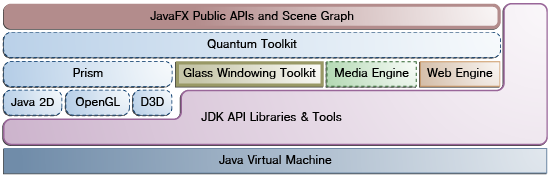
\includegraphics[scale=0.7]{Gambar/arsitekturJavaFX}
	\caption{Arsitektur JavaFX}
	\end{figure}
	
Ilustrasi dari gambar \textbf{2.1} mendeskripsikan setiap komponen saling berhubungan. Dibawah JavaFX Public API terdapat mesin yang menjalankan code JavaFX. Mesin tersebut terdiri dari sub komponen termasuk mesin grafis berperforma tinggi yang dinamakan Prism. Selain itu, terdapat sistem \textit{windowing} kecil dan efisien yang dinamakan Glass. Terakhir dalam mesin dibawah JavaFX Public API terdapat sebuah \textit{media engine} dan \textit{web engine}. Berikut ini elemen-elemen yang terdapat pada arsitektur JavaFX : \cite{javafx}
\begin{enumerate}
	\item \textit{Scene Graph}
	\item Java Public API untuk Fitur JavaFX
	\item \textit{Graphics System}
	\item \textit{Glass Windowing Toolkit}
	\item Gambar dan Media
	\item Komponen Web
	\item CSS
	\item \textit{UI Control}
	\item Layout
	\item Transformasi 2-D dan 3-D
	\item \textit{Visual Effecs}
\end{enumerate}

\subsection{Scene Graph}
\label{subs:Scene_Graph}
\textit{Scene Graph} merupakan sebuah pohon hirarki dari sekumpulan node yang merepresentasikan elemen visual dari antarmuka suatu aplikasi. Sebuah elemen dari \textit{scene graph} dinamakan node. Setiap node mempunya ID, \textit{style class} dan \textit{boundling volume}. Node dalam \textit{scene graph} juga memiliki :\cite{javafx}
\begin{enumerate}
	\item \textit{Effect}, seperti blur dan shadow
	\item \textit{Opacity}
	\item \textit{Transform}
	\item \textit{Event handler} (Mouse, keyboard, dan input method lainnya)
	\item Perintah spesifik dari sebuah aplikasi
\end{enumerate} 

Penggunaan \textbf{javafx.scene} API memungkinkan \textit{developer} untuk menggunakan beberapa jenis konten dialamnya, seperti : \cite{javafx}
\begin{enumerate}
	\item \textbf{Node} : Bentuk(2-D dan 3-D), gambar, media, \textit{embedded web browser}, teks, \textit{UI control}, grafik, grup, dan \textit{container}.
	\item \textbf{State} : Transformasi (posisi dan orientasi dari node), efek visual, dan konten visual lainnya.
	\item \textbf{Effect} : objek sederhana yang dapat merubah penampilan dari node \textit{scene graph}, seperti blur, shadow, dan \textit{color adjustment}
\end{enumerate}

\subsection{Java Public API untuk Fitur JavaFX}
\label{subs:API}
Pada lapisan atas arsitektur JavaFX pada gambar \textbf{2.1} API Java memberikan kebebasan dan fleksibilitas untuk membangun berbagai \textit{client} dari sebuah aplikasi. Platform JavaFX menggabungkan kemampuan terbaik yang dimiliki platform Java secara menyeluruh dan mendalam serta intuitif dengan memasukan fungsi media kedalamnya, sehingga tercipta lingkup konsep \textit{one-stop development}. Berikut contoh kegunaan Java API untuk fitur JavaFX :\cite{javafx}
\begin{enumerate}
	\item Memungkinkan penggunaan fitur Java yang poweful seperti \textit{generics, annotations, multithreading}.
	\item Lebih mudah mengembangan web menggunakan JavaFX dibanding \textit{JVM-base dynamic languages} lainnya seperti Grovvy, dan JavaScript.
	\item Memungkinkan Java developer untuk menggunakan bahasa sistem seperti Groovy untuk menulis file besar atau kompleks pada aplikasi JavaFX.
	\item Memungkinkan penggunaan binding.
	\item Menambahkan koleksi library Java dengan memasukan urutan dan memetakan perubahan sehingga memngukinkan aplikasi untuk menghubungkan antarmuka kedalam data model, mengamati perubahan pada data model, dan memperbarui kontrol UI yang sesuai dengan perubahan tersebut.   
\end{enumerate}

\subsection{Graphic System}
\label{subs:Graphic_System}
\textit{JavaFX Graphic System} pada gambar \textbf{2.1} merupakan implementasi dari JavaFX \textit{scene graph layer}. Sistem grafis pada JavaFX mendukung tampilan 2-D dan 3-D, selain itu sistem grafis ini menyediakan \textit{software rendering} untuk mendukung akselerasi \textit{rendering} dari \textit{hardware}. Berukut ini merupakan dua \textit{graphic accelerated pipeline} yang ada pada JavaFX platform :\cite{javafx}
\begin{enumerate}
	\item \textbf{Prism} yang bekerja pada proses render. Prism dapat bekerja pada kedua sisi baik \textit{hardware} maupun \textit{software} rendering termasuk 3-D rendering. Prism juga bertanggung jawab untuk proses \textit{rasterization}(mengubah vektor menjadi pixel atau dot) dan rendering pada JavaFX.
	\item \textbf{Quantum Toolkit} merupakan perpaduan Prism dan Windowing Toolkit yang bekerja di lapisan teratas pada JavaFX untuk mengatur \textit{threading rule} yang berhubungan dengan rendering dan \textit{event handling}. 
\end{enumerate}

\subsection{Glass Windowing Toolkit}
\label{subs:Glass_Windowing_Toolkit}
Tugas pada lapisan ini adalah membantu \textit{service} pada sistem operasi, seperti mengatur windows, waktu , dan \textit{surface}. Glass Toolkit juga bertanggung jawab atas pengaturan \textit{event queue}.\cite{javafx}

\subsection{Media dan Gambar}
\label{subs:Media_Gambar}
Fungsi -fungsi media pada JavaFX tersedia pada \textbf{javafx.scene.media} API. JavaFX mensuport baik visual maupun audio. Beberapa format yang disuport seperti MP3, AIFF, WAV pada file audio dan format FLV pada video. Ada tiga komponen yang berperan pada JavaFX media, yaitu :\cite{javafx} 
\begin{enumerate}
	\item \textit{Media object} merepresentasikan sebuah file media.
	\item \textit{Media Player} memutar sebuah file media.
	\item \textit{Media View} merupakan sebuah node yang menampilkan media tersebut.
\end{enumerate}

\subsection{Komponen Web}
\label{subs:Komponen_Web}
Mesin Web pada JavaFX merupakan bagian dari JavaFX UI control yang berbasis Webkit, dimana mesin web ini dapat menampilkan sebuah website dan melakukan browsing melalui APInya. Berikut ini fitur JavaFX yang dapat di implementasikan pada program java :\cite{javafx}
\begin{enumerate}
	\item Render konten HTML dari local atau remote URL.
	\item Mendukung history dan menyediakan navigasi Back dan Forward.
	\item \textit{Reload Content}.
	\item Edit konten HTML.
	\item Mengeksekusi perintah JavaScript.
	\item \textit{Handle event}.
\end{enumerate} 

Komponen dari browser tersebut terbagi kedalam ke kelas-kelas berikut :\cite{javafx}
\begin{enumerate}
	\item \textbf{WebEngine} : menyediakan kemampuan dasar dari halaman web.
	\item \textbf{WebView} : merangkum sebuah \textit{WebEngine object}, Menggabungkan konten HTML kedalam layar aplikasi, dan mendukung \textit{field} dan \textit{method} untuk menerapkan efek dan transformasi berupa ekstensi maupun sebuah kelas Node.
\end{enumerate}

\subsection{CSS}
\label{subs:CSS}
JavaFX Cascading Style Sheet (CSS) mendukung kemampuan untuk mengkustom styling pada antarmuka sebuah aplikasi JavaFX tanpa merubah \textit{source code} aplikasi tersebut.\cite{javafx}   

\subsection{UI Control}
\label{subs:UI_Control}
JavaFX UI Control dalam JavaFX API dibangun menggunakan node pada scene graph. JavaFX UI Control dapat mengambil keuntungan dari fitur yang diberikan platform JavaFX dan bersifat \textit{portable} pada platform yang berbeda.\cite{javafx}

\begin{figure}[H]
	\centering
	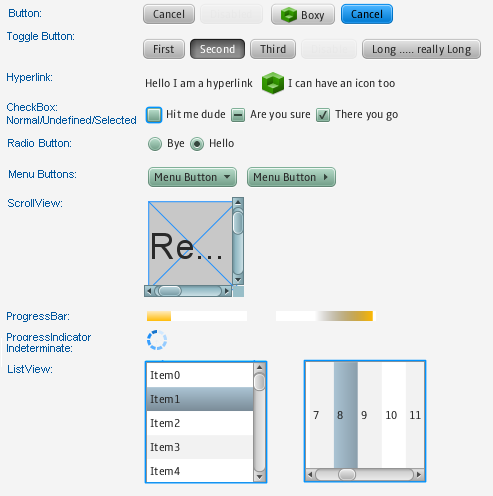
\includegraphics[scale=0.8]{Gambar/JavaFXuicontrols}
	\caption{Contoh JavaFX UI Control}
	\end{figure}
	
	pada gambar \textbf{2.2} menunjukan UI Control yang sementara didukung oleh JavaFX. Java UI control baru seperti TitlePane atau Accordion sebelumnya telah diperkenalkan pada JavaFX SDK. UI control tersebut terdapat pada \textbf{javafx.scene.control} \textit{package}.\cite{javafx}
 
\subsection{Layout}
\label{subs:Layout}
 \textit{Layout container} atau panel digunakan untuk pengatruan UI control secara dinamis dan fleksibel dalam scene graph pada aplikasi JavaFX. JavaFX Layout API mempunyai kelas-kelas yang dapat mengotomatiskan tata letak model sebagai berikut:\cite{javafx}
\begin{enumerate}
	\item \textbf{BorderPane} merupakan kelas yang mengatur bagian atas, bawah, kiri, kanan layout.
	\item \textbf{Hbox} merupakan kelas yang mengatur konten node secara horizontal dalam satu baris.
	\item  \textbf{Vbox} merupakan kelas yang mengatur konten node secara vertikal dalam satu baris.
	\item \textbf{StackPane} adalah kelas yang menempatkan \textit{back-to-front} konten node pada suatu \textit{stack}.
	\item \textbf{GridPane} adalah kelas yang memungkinkan developer untuk membuat sebuah grid baris dan kolom secara flexible untuk memetakan konten node.
	\item \textbf{FlowPane} adalah kelas yang mengatur alur konten node baik horizontal maupun vertical, \textit{wrapping} pada batas lebar konten (untuk horizontal) atau tinggi konten (untuk vertical).
	\item \textbf{AnchorPane} adalah kelas yang memungkinkan developer untuk membuat \textit{anchor} node pada layout atas, bawah, sisi kiri atau ditengah layout. 
\end{enumerate}

\subsection{Transformasi 2-D dan 3-D}
\label{subs:Layout}
Setiap node pada JavaFX scene graph dapat ditransformasikan dalam koordinat x-y melalui kelas-kelas \textit{javafx.scene.transform} berikut ini:\cite{javafx}
\begin{enumerate}
	\item \textbf{translate} - Memindahkan sebuah node dari satu posisi ke posisi lain bersama koordinat x,y,z yang relatif terhadap posisi awalnya.
	\item \textbf{scale} - Meresize sebuah node untuk membesar atau mengecil sesuai koordinat x,y,z tergantung skala faktornya.
	\item \textbf{rotate} - Merotasi sebuah node sesuai titik porosnya.
	\item \textbf{affine} - Melakukan pemetaan linear dari koordinat 2-D / 3-D ke koordinat 2-D / 3-D lainnya dengan menjaga lurus dan paralel sifat garis tersebut. Kelas ini digunakan bersamaan dengan kelas lainya dibanding penggunaan langsung.
\end{enumerate}

\subsection{Komponen JavaFX}
\label{subs:Komponen_Java_FX}
Berikut ini merupakan kumpulan \textit{package} yang ada dalam JavaFX.\cite{javafx3}
\begin{table}[H]
		\centering
		\caption{Tabel komponen JavaFX}
		\label{tab:komponen_javafx}
	\begin{tabular}{|c|p{12cm}|}
		\hline
		\textbf{No} & \textbf{Package dan Deskripsi} \\ \hline \hline
		1 & \textbf{javafx.application}\\
			&	Menyediakan kelas-kelas dalam siklus aplikasi.\\ \hline
		2 & \textbf{javafx.event}\\
			&	Memberikan kerangka dasar untuk FX event, dari mulai pengiriman hingga handling.\\ \hline	
		3 & \textbf{javafx.fxml}\\
			&	Berisi kelas untuk membuat hirarki objek dari markup.\\ \hline
		4 & \textbf{javafx.scene}\\
			&	Memberikan set basis kelas - kelas untuk JavaFX Scene Graph API .\\ \hline
		5 & \textbf{javafx.scene.control}\\
			&	JavaFX \textit{User Interface Control }(kontrol UI atau kontrol saja) dimana node khusus dalam JavaFX Scenegraph yang dapak digunakan untuk banuak konteks aplikasi yang berbeda.\\ \hline
		6 & \textbf{javafx.scene.input}\\
			&	Menyediakan set kelas - kelas untuk mouse dan keyboard \textit{input event handling}.\\ \hline
		7 & \textbf{javafx.scene.layout}\\
			&	Menyediakan kelas - kelas untuk mendukung UI layout.\\ \hline
		8 & \textbf{javafx.scene.text}\\
			&	Menyediakan set kelas - kelas untuk font dan teks node yang dapat di render.\\ \hline
		9 & \textbf{javafx.util}\\
			&	Berisi berbagai utilitas dan kelas pembantu.\\ \hline
		10 & \textbf{javafx.util.converter}\\
			&	\textit{Package} ini untuk konversi String pada JavaFX.\\ \hline
		11 & \textbf{javafx.beans}\\
			&	\textit{Package} ini berisi interface yang mendefinisikan bentuk umum dari \textit{observability}.\\ \hline
		12 & \textbf{javafx.beans.binding}\\
			&	\textit{Package} ini untuk menjelaskan karakter dari \textit{Binding}.\\ \hline	
		13 & \textbf{javafx.beans.value}\\
			&	\textit{Package} ini berisi fundamental interface dari \textit{observableValue} dan \textit{WritebleValue} dan semua sub interface di dalamnya.\\ \hline
		14 & \textbf{javafx.collections}\\
				&	\textit{Package} ini berisi koleksi penting dari javaFX dan koleksi utilitas lainnya.\\ \hline						
	\end{tabular}
\end{table}
\subsection{Property}
Properti merupakan \textit{interface} generik yang mendefinisikan metode umum untuk sifat yang dapat ditulis secara independen sesuai tipenya.\cite{javafx3}
\subsection{javafx.collections}
\subsubsection{ObservableList}
Dalam \textit{package} javafx.collections terdapat sebuah \textit{interface} yang bernama ObservableList. \textit{Interface} ini merupakan sebuah \textit{list} yang memungkinkan \textit{listeners} melacak ketika terjadi perubahan pada \textit{list} tersebut.
. Berikut ini \textit{method} yang ada pada \textit{interface} ObservableList.\cite{javafx3}
\begin{table}[H]
		\centering
		\caption{Tabel method ObservableList}
		\label{tab:method_ObservableList}
	\begin{tabular}{|c|p{12cm}|}
		\hline
		\textbf{No} & \textbf{Method dan Deskripsi} \\ \hline \hline
		1 & \textbf{addAll(E... elements)}\\
			&	Sebuah metode untuk menambah semua variabel dari sebuah elemen.\\ \hline
		2 & \textbf{addListener(ListChangeListener<? super E> listener)}\\
			&	Menambahkan \textit{listeners} pada sebuah observableList.\\ \hline
	\end{tabular}
\end{table}

\subsubsection{ListChangeListener}
\textit{Interface} ini menerima informasi perubahan dari sebuah ObservableList. Berikut ini \textit{method} yang ada pada \textit{interface} ListChangeListener.\cite{javafx3}
\begin{table}[H]
		\centering
		\caption{Tabel method ListChangeListener}
		\label{tab:method_ListChangeListener}
	\begin{tabular}{|c|p{12cm}|}
		\hline
		\textbf{No} & \textbf{Method dan Deskripsi} \\ \hline \hline
		1 & \textbf{onChanged(ListChangeListener.Change<? extends E> c)}\\
			&	Metode ini dipanggil ketika perubahan telah dilakukan terhadap sebuah ObservableList.\\ \hline
	\end{tabular}
\end{table}

\subsection{javafx.scene.control}
JavaFX UI \textit{control}(kontrol UI atau Kontrol) merupakan Node khusus pada JavaFX \textit{scenegraph} yang dapat digunakan berulang kali menyesuaikan kebutuhan rancangan aplikasi. Kontrol UI dapat disesuaikan visualnya oleh desainer atau pengembang aplikasi. \textit{Interface} ini didesain untuk berkerja dalam \textit{layout system}. Contoh \textit{interface} ini adalah Button, Label, ListView, TableView, dan TextField.\cite{javafx3}

\subsubsection{TextField}
TextField merupakan komponen \textit{input} teks yang memungkinkan pengguna untuk memasukan satu baris teks terformat. Berikut ini \textit{method} pada kelas TextField.\cite{javafx3}
\begin{table}[H]
		\centering
		\caption{Tabel method TextField}
		\label{tab:method_textField}
	\begin{tabular}{|c|p{12cm}|}
		\hline
		\textbf{No} & \textbf{Method dan Deskripsi} \\ \hline \hline
		1 & \textbf{getOnAction()}\\
			&	Metode ini menangani aksi terkait \textit{text field} ini. Method ini mengembalikan nilai null bila tidak ada aksi yang diberikan.\\ \hline
	\end{tabular}
\end{table}

\subsubsection{TableView}
TableView dirancang untuk memvisualisasikan jumlah baris data. Jumlah baris data tersebut akan dipecah menjadi kolom-kolom dalam TabelView. Berikut \textit{method} dalam kelas TabelView.\cite{javafx3}

\begin{table}[H]
		\centering
		\caption{Tabel method TabelView}
		\label{tab:method_TabelView}
	\begin{tabular}{|c|p{12cm}|}
		\hline
		\textbf{No} & \textbf{Method dan Deskripsi} \\ \hline \hline
		1 & \textbf{setItems(ObservableList<S> value)}\\
			&	Menetapkan nilai dari properti item pada tabel.\\ \hline
		2 & \textbf{getOnSort()}\\
			&	\textit{Method} ini dipanggil ketika ada permintaan untuk \textit{sorting}.\\ \hline		
	\end{tabular}
\end{table}

\subsubsection{TableColumn}
Sebuah TableView terdiri dari sejumlah TableColumn. Setiap TableColumn pada tabel bertanggung jawab menampilkan dan mengedit isi kolom. Berikut \textit{method} pada TableColumn.\cite{javafx3}
\begin{table}[H]
		\centering
		\caption{Tabel method TableColumn}
		\label{tab:method_TableColumn}
	\begin{tabular}{|c|p{14cm}|}
		\hline
		\textbf{No} & \textbf{Method dan Deskripsi} \\ \hline \hline
		1 & \textbf{setCellValueFactory(Callback<TableColumn.CellDataFeatures<S,T>}\\
			& \textbf{,ObservableValue<T>> value)}\\
			&	Menetapkan nilai properti \textit{CellFactory} yang dibutuhkan untuk menentukan bagaimana sel terisi pada satu TableColumn .\\ \hline	
	\end{tabular}
\end{table}
